\begingroup
\clearpage
\let\clearpage\relax
\vspace*{-16pt}
\chapter[COMPUTATIONAL STUDY]{COMPUTATIONAL STUDY}\label{sec.results}
\endgroup

This chapter presents the computational results for the solution
methods developed in Chapter~\ref{sec.methods}, evaluated on the testbed described in Chapter~\ref{sec.DATAPREP}. The experiments cover
instances sampled from the MIMIC-IV cohort of \numprint{223291}
patients, with cohort sizes ranging from \numprint{1000} to
\numprint{30000} patients. We compare exact combinatorial algorithms,
direct MILP formulations with implementation enhancements, and
variants of the LBBD algorithm. All experiments were conducted on a high-performance compute node with an Intel Xeon Gold 6130F CPU @ 2.10~GHz and 1.5~TB RAM, using Gurobi 12.0.0 as the MILP solver. All algorithms and methods were implemented in Python 3.9.23. A time limit of \numprint{7200} seconds (2 hours) was imposed for all methods, and running times are reported in seconds. Delayed constraint addition is implemented via Gurobi's lazy cut functionality.

The frequency threshold $\ell = 100$ is used throughout, chosen after
preliminary experimentation. In practice, $\ell$ should be set to a
sufficiently large fraction of $|P|$ to ensure statistical reliability
of the mortality rate estimate. As mentioned in Chapter~\ref{sec.probstmnt}, every vertex
$u$ with $|A_u| \le \ell - 1$ and every edge $\{u,v\}$ with
$|A_u \cap A_v| \le \ell - 1$ are removed from the comorbidity graph,
so that $|A_u| \ge \ell$ for each $u \in V$ and
$|A_u \cap A_v| \ge \ell$ for each $\{u,v\} \in E$.

The results are organized as follows. Section~\ref{sec.CCA} compares
the modified Bron--Kerbosch and combinatorial branch-and-bound
algorithms. Section~\ref{sec.milp-dcg} evaluates the two MILP
formulations and their implementation variants.
Section~\ref{sec.lbbds} compares the pure and hybrid LBBD algorithms.
Section~\ref{sec.sidecons} demonstrates the extensibility of the LBBD
framework through a case study incorporating an age-based side
constraint. Section~\ref{sec.exp2-BKscalability} evaluates the
scalability of the modified Bron--Kerbosch algorithm on the full
MIMIC-IV dataset, and Section~\ref{sec.exp3-margMR} presents a
sensitivity analysis and marginal mortality rate experiments. Detailed
results are provided in Appendix~\ref{App.tableDeets}.

The following column headings are used throughout the tables. ``Size''
reports the patient cohort size, and ``No.'' the sample identifier within
a cohort size. ``Clique'' lists the diseases comprising the reported
clique, with disease names abbreviated; full names are provided in
Appendix~\ref{App.Abbs}. ``$\mu$'' denotes the mortality rate of a clique,
and ``Increase'' the percentage by which the mortality rate rises when the
indicated disease or diseases are added to an initial clique. ``Best Obj''
reports the best objective value (mortality rate) found. ``Time'' reports
wall-clock running time rounded down to the nearest second; an entry of
``TO'' indicates that the time limit was reached. ``Gap'' reports the
percentage optimality gap at termination, with zero indicating optimality
within solver tolerance. In LBBD tables, ``\#Opt Cuts'', ``\#Feas Cuts'',
and ``\#CBB Cuts'' report the number of optimality cuts, feasibility cuts,
and CBB cuts added, respectively. In summary tables, ``Avg'' and ``Range''
give the average and the minimum--maximum range across the five samples for
each cohort size.

\section{Comparing Combinatorial Algorithms}\label{sec.CCA}

Table~\ref{tab.SBKCBB} summarizes the results comparing the modified
Bron--Kerbosch algorithm (Algorithm~\ref{alg.BKMMRC}) and the CBB algorithm
(Algorithm~\ref{alg.CBB}). Detailed sample-wise results appear in
Table~\ref{tab.BKCBB} in the appendix. Both methods guarantee
optimality unless the time limit is reached. The column ``\#RC
decrease'' reports the average reduction in recursive calls
attributable to the $\gamma$-upper-bound pruning~\eqref{eq.gammaC}
in the CBB algorithm, which is the primary differentiator between the
two methods.

Both methods solve all tested instances up to \numprint{30000}
patients. For the BK algorithm, average running times increase from
under 1 second for \numprint{1000}-patient instances to approximately
73 seconds for \numprint{30000}-patient instances. The CBB algorithm
is considerably faster: its average running time remains below 1
second for instances with up to \numprint{5000} patients, rises to 1
second at \numprint{10000} patients, 3 seconds at \numprint{15000}
patients, 8 seconds at \numprint{20000} patients, 22 seconds at
\numprint{25000} patients, and 2 seconds at \numprint{30000} patients.
The number of recursive calls grows with instance size for the BK
algorithm, while the CBB algorithm requires far fewer. The average
reduction in recursive calls ranges from 28 for \numprint{1000}-patient
instances to \numprint{1153091} for \numprint{30000}-patient instances.
The average maximum mortality rate across instances ranges from 0.45
at \numprint{1000} patients to 0.97 at \numprint{25000} patients,
with a value of 0.85 at \numprint{30000} patients. The full
\numprint{223291}-patient instance exceeds the time limit for both
algorithms.  
\begin{table}[htpb]
\centering
\resizebox{\textwidth}{!}{\begin{tabular}{rrrrrrrrr}
\toprule
Size & \multicolumn{2}{c}{Best Obj} & \multicolumn{2}{c}{BK, Time} &
\multicolumn{2}{c}{CBB, Time} & \#RC decrease\\
 & Avg & Range & Avg & Range & Avg & Range & Avg \\
\midrule
\numprint{1000} & 0.45 & [0.41, 0.49] & $<1$ & [$<1$, $<1$] & $<1$ &
[$<1$, $<1$] & 28 \\
\numprint{5000} & 0.80 & [0.72, 0.88] & 1 & [1, 1] & $<1$ & [$<1$,
$<1$] & \numprint{2207}\\
\numprint{10000} & 0.86 & [0.81, 0.92] & 2 & [2, 3] & 1 & [1, 1] &
\numprint{20787}\\
\numprint{15000} & 0.95 & [0.89, 1.00] & 8 & [5, 9] & 3 & [2, 4] &
\numprint{89191}\\
\numprint{20000} & 0.97 & [0.96, 0.99] & 24 & [22, 27] & 8 & [7, 8] &
\numprint{241932} \\
\numprint{25000} & 0.97 & [0.97, 0.98] & 47 & [42, 53] & 22 & [20,
26] & \numprint{478683}\\
\numprint{30000} & 0.85 & [0.83, 0.88] & 73 & [66, 83] & 2 & [2, 2] &
\numprint{1153091}\\
\numprint{223291} & UNK\footnotemark & UNK & TO & UNK & UNK & TO & UNK\\
\bottomrule
\end{tabular}}
\caption{\label{tab.SBKCBB} Comparing Modified Bron--Kerbosch and CBB Algorithms}
\end{table}

\footnotetext{UNK stands for Unknown (no value was reported because the run timed out).}

\section{Comparing MILP Solutions}\label{sec.milp-dcg}

We implemented formulation~\eqref{form.milp} using delayed addition of
the linearizing constraints~\eqref{eq.wto0}--\eqref{eq.wtozUB}, which
scale with $|P|$. All violated constraints of this type are added at
BC nodes where an integral solution is encountered as the node LP
relaxation optimum. Preliminary experiments showed this to perform
better than delaying
constraints~\eqref{eq.xyconnectupper-disagg}--\eqref{eq.xyconnectlowerFP}.
We also explored an implementation using an aggregated variant of
constraints~\eqref{eq.xyconnectupper-disagg}, given by
constraint~\eqref{eq.xyconnectupperagg}, in the root LP formulation.
This aggregated form models the requirement as
\begin{align}
    |V \setminus D_i| y_i &\le |V \setminus D_i| - \sum_{j \in V
    \setminus D_i} x_j & \forall i \in P.
    \label{eq.xyconnectupperagg}
\end{align}
Formulation~\eqref{form.CCIP} was implemented using Gurobi's indicator
constraint feature~\citep{gurobi-indicator} for
constraints~\eqref{eq.xlin1CC}--\eqref{eq.xlin3CC}, which model the
products $\bar{x}_u = x_u \cdot t$. These indicator constraints
directly encode the implication that $x_u = 1$ forces $\bar{x}_u = t$
and $x_u = 0$ forces $\bar{x}_u = 0$, without requiring explicit
big-M coefficients. Gurobi internally generates an equivalent MIP
representation during the solution process.
Constraints~\eqref{eq.xyconnectupper-disaggcc}--\eqref{eq.xyconnectlowerFPcc}
are also added in a delayed manner at BC nodes with integral LP optima.

Detailed results comparing formulation~\eqref{form.milp} with
aggregation, formulation~\eqref{form.milp} without aggregation, and
formulation~\eqref{form.CCIP} are reported in Table~\ref{tab.MILPs}
in the appendix. All three formulations solve the
\numprint{1000}-patient instances to optimality: formulation
\eqref{form.milp} with aggregation requires 16--35 seconds per sample,
without aggregation requires 66--75 seconds, and
formulation~\eqref{form.CCIP} requires 2--4 seconds.

Only formulation~\eqref{form.CCIP} consistently solves the
\numprint{5000}-patient instances to optimality. Both variants of
formulation~\eqref{form.milp} reach the time limit with optimality
gaps of 13\%--54\% with aggregation and 13\%--47\% without. For
instances with \numprint{10000} patients or more, all three
formulations reach the time limit on nearly all instances.

\section{Comparing LBBD Variants}\label{sec.lbbds}

In this section, we compare the performance of the two LBBD variants, pure LBBD and hybrid
LBBD. Pure LBBD is the DBC algorithm from
Section~\ref{sec.gamma-lbbd}, using the separation procedure in
Algorithm~\ref{alg.LBBDgamma} at BC nodes where the LP relaxation
optimum is integral. Hybrid LBBD is the algorithm from
Section~\ref{sec.hybridLBBD}, using Algorithm~\ref{alg.hybridLBBD}
instead, and adding CBB cuts at BC nodes where the incumbent
$\ell$-frequent clique contains at least $\tau$ vertices. The root
relaxation is additionally strengthened with CBB cuts generated from
$k$ calls to the CBB algorithm, one for each of the $k$ diseases with
the highest individual mortality rate. Constraint~\eqref{eq.zmuLB} is
updated if a better lower bound is found among the resulting cliques.
Based on preliminary experimentation, we set $\tau = 4$ and $k = 5$
for all experiments.

\begin{table}[htpb]
\centering
\resizebox{\textwidth}{!}{\begin{tabular}{rrrrrrrrr}
 \toprule
Size & \multicolumn{2}{c}{Gap} & \multicolumn{2}{c}{Time} &
\multicolumn{2}{c}{\#Opt Cuts} & \multicolumn{2}{c}{\#Feas Cuts} \\
 & Avg & Range & Avg & Range & Avg & Range & Avg & Range \\
\midrule
\numprint{1000} & 0 & [0, 0] & $<1$ & [$<1$, $<1$] & 13.6 & [4, 21]
& 52.4 & [18, 92]\\
\numprint{5000} & 0 & [0, 0] & 3 & [2, 4] & \numprint{1051} & [783,
\numprint{1365}] & 778.4 & [577, \numprint{1039}]\\
\numprint{10000} & 0 & [0, 0] & 296 & [240, 378] & \numprint{15633} &
[\numprint{11427}, \numprint{19593}] & \numprint{14211} &
[\numprint{12036}, \numprint{16057}]\\
\numprint{15000} & 3 & [0, 6] & TO & [47, TO] & \numprint{60683} &
[\numprint{5010}, \numprint{92190}] & \numprint{52675} &
[\numprint{4452}, \numprint{74083}]\\
\numprint{20000} & 3 & [1, 4] & TO & [TO, TO] & \numprint{72174} &
[\numprint{62069}, \numprint{85761}] & \numprint{72691} &
[\numprint{62164}, \numprint{82328}] \\
\numprint{25000} & 3 & [2, 4] & TO & [TO, TO] & \numprint{65231} &
[\numprint{49369}, \numprint{82039}] & \numprint{76147} &
[\numprint{59438}, \numprint{89502}]\\
\numprint{30000} & 3 & [3, 5] & TO & [TO, TO] & \numprint{61358} &
[\numprint{56441}, \numprint{75841}] & \numprint{137369} &
[\numprint{114797}, \numprint{150718}]\\
\numprint{223291} & 3 & & TO & & \numprint{58825} & & \numprint{42595}
&\\
 \bottomrule
\end{tabular}}
  \caption{\label{tab.SumG} Summary of Results from the Pure LBBD}
\end{table}

\begin{table}[htpb]
 \centering
\resizebox{\textwidth}{!}{\begin{tabular}{rrrrrrrrrrr}
 \toprule
Size & \multicolumn{2}{c}{Gap} & \multicolumn{2}{c}{Time} &
\multicolumn{2}{c}{\#Opt Cuts} & \multicolumn{2}{c}{\#Feas Cuts} &
\multicolumn{2}{c}{\#CBB Cuts}\\
 & Avg & Range & Avg & Range & Avg & Range & Avg & Range & Avg &
 Range\\
\midrule
\numprint{1000} & 0 & [0, 0] & $<1$ & [$<1$, $<1$] & 8.6 & [5, 14] &
0 & [0, 0] & 0 & [0, 0]\\
\numprint{5000} & 0 & [0, 0] & 1 & [1, 2] & \numprint{912} &
[\numprint{736}, \numprint{1249}] & \numprint{566} & [\numprint{507},
\numprint{645}] & 63 & [4, \numprint{183}]\\
\numprint{10000} & 0 & [0, 0] & 100 & [64, \numprint{146}] &
\numprint{9053} & [\numprint{7762}, \numprint{10571}] & \numprint{7062}
& [\numprint{4764}, \numprint{9619}] & \numprint{4599} &
[\numprint{2527}, \numprint{6842}]\\
\numprint{15000} & 0 & [0, 0] & \numprint{1283} & [7, \numprint{2394}]
& \numprint{26169} & [\numprint{577}, \numprint{39564}] & \numprint{4118}
& [45, \numprint{7257}] & \numprint{21731} & [\numprint{189},
\numprint{34797}]\\
\numprint{20000} & 2 & [0, 4] & TO & [TO, TO] & \numprint{81976} &
[\numprint{79347}, \numprint{89610}] & \numprint{72336} &
[\numprint{70127}, \numprint{76794}] & \numprint{44145} &
[\numprint{41677}, \numprint{48648}]\\
\numprint{25000} & 2 & [1, 3] & TO & [TO, TO] & \numprint{74992} &
[\numprint{62595}, \numprint{82335}] & \numprint{76783} &
[\numprint{66641}, \numprint{86002}] & \numprint{43782} &
[\numprint{37470}, \numprint{48200}]\\
\numprint{30000} & 0 & [0, 0] & \numprint{716} & [\numprint{532},
\numprint{1102}] & \numprint{19945} & [\numprint{18620},
\numprint{22737}] & \numprint{24769} & [\numprint{23116},
\numprint{26965}] & \numprint{7158} & [\numprint{6476},
\numprint{8336}]\\
\numprint{223291} & 2 & & TO & & \numprint{423} & & 1 & & 201 &\\
 \bottomrule
\end{tabular}}
\caption{\label{tab.SumH} Summary of Results from the Hybrid LBBD Algorithm}
\end{table}

Tables~\ref{tab.SumG} and~\ref{tab.SumH} summarize the results for
the two LBBD variants; sample-wise details appear in
Tables~\ref{tab.Gam} and~\ref{tab.HybridLBBD} in
Appendix~\ref{App.tableDeets}. Both variants solve the
\numprint{1000}-patient and \numprint{5000}-patient instances quickly:
pure LBBD takes an average of under 1 second and 3 seconds,
respectively, while hybrid LBBD takes under 1 second and 1--2
seconds. On \numprint{10000}-patient instances, both variants solve
all five instances to optimality; hybrid LBBD requires an average of
100 seconds, approximately one third of the 296-second average for
pure LBBD. For \numprint{15000}-patient instances, pure LBBD solves
two instances to optimality (in 47 and \numprint{2278} seconds) and
reaches the time limit on the remaining three with gaps between
0\% and 6\%, while hybrid LBBD solves all five to optimality with an
average of \numprint{1283} seconds.

Both variants reach the time limit on all \numprint{20000}-patient and
\numprint{25000}-patient instances. The pure LBBD reports an average
gap of 3\% at both sizes,
while hybrid LBBD reports an average gap of 2\%. For \numprint{30000}-patient instances, pure LBBD reaches
the time limit on all instances with an average gap of 3\%, while hybrid LBBD solves all five to optimality with an
average of 716 seconds. On the
full \numprint{223291}-patient instance, both variants reach the time
limit; pure LBBD reports a gap of 3\% and hybrid LBBD reports a gap
of 2\%. Overall, the hybrid LBBD algorithm is substantially faster on
instances up to \numprint{15000} patients and is the only method that
solves all \numprint{30000}-patient instances to optimality. Detailed numerical results for all instances and all algorithms are
provided in Appendix~\ref{App.tableDeets}.

\section{Side Constraints and the Hybrid LBBD
Algorithm}\label{sec.sidecons}
An important feature of the LBBD framework is that it is grounded in
integer programming, which allows additional constraints on the $x$
variables to be incorporated into $\calX$ with relative ease. This
contrasts with the CBB algorithm, which may require substantial
modifications to accommodate new constraints. Importantly, the CBB
cut remains valid in the presence of new constraints in $\calX$,
since it still provides a valid upper bound on the optimal solution,
and the hybrid LBBD algorithm continues to be applicable. To
illustrate this, we consider two case studies. In Section~\ref{sec.AgeSide}, an age-based side
constraint is added to the original problem. In Section~\ref{sec.CancerSide}, we incorporate a constraint
requiring the selected clique to contain at least one cancerous
diagnosis, directing the search toward high-mortality clusters
that include cancer as a component.

\subsection{Case Study: Limiting Age-Associated Diseases} \label{sec.AgeSide}

In practice, older patients tend to exhibit more comorbidities and
higher baseline mortality, which can influence the composition of
maximum mortality rate cliques. We define a practical age threshold
of 60, and for each disease $v \in V$ compute the proportion of its
patients who are 60 or older:
\begin{align*}
    a_{60}(v) &\coloneqq \frac{|\{i \in A_v : \text{age}(i) \ge
    60\}|}{|A_v|}, \qquad \forall v \in V.
\end{align*}
We then impose constraint~\eqref{eq.oldagecon}, which limits the
average $a_{60}(v)$ across selected diseases to at most 0.5, with the
aim of identifying high-mortality cliques whose lethality is not
primarily attributable to an older patient composition:
\begin{equation}\label{eq.oldagecon}
    \sum_{v \in V} a_{60}(v) x_v \;\le\; 0.5\,\sum_{v \in V} x_v.
\end{equation}

\begin{figure}[htbp]
    \centering
    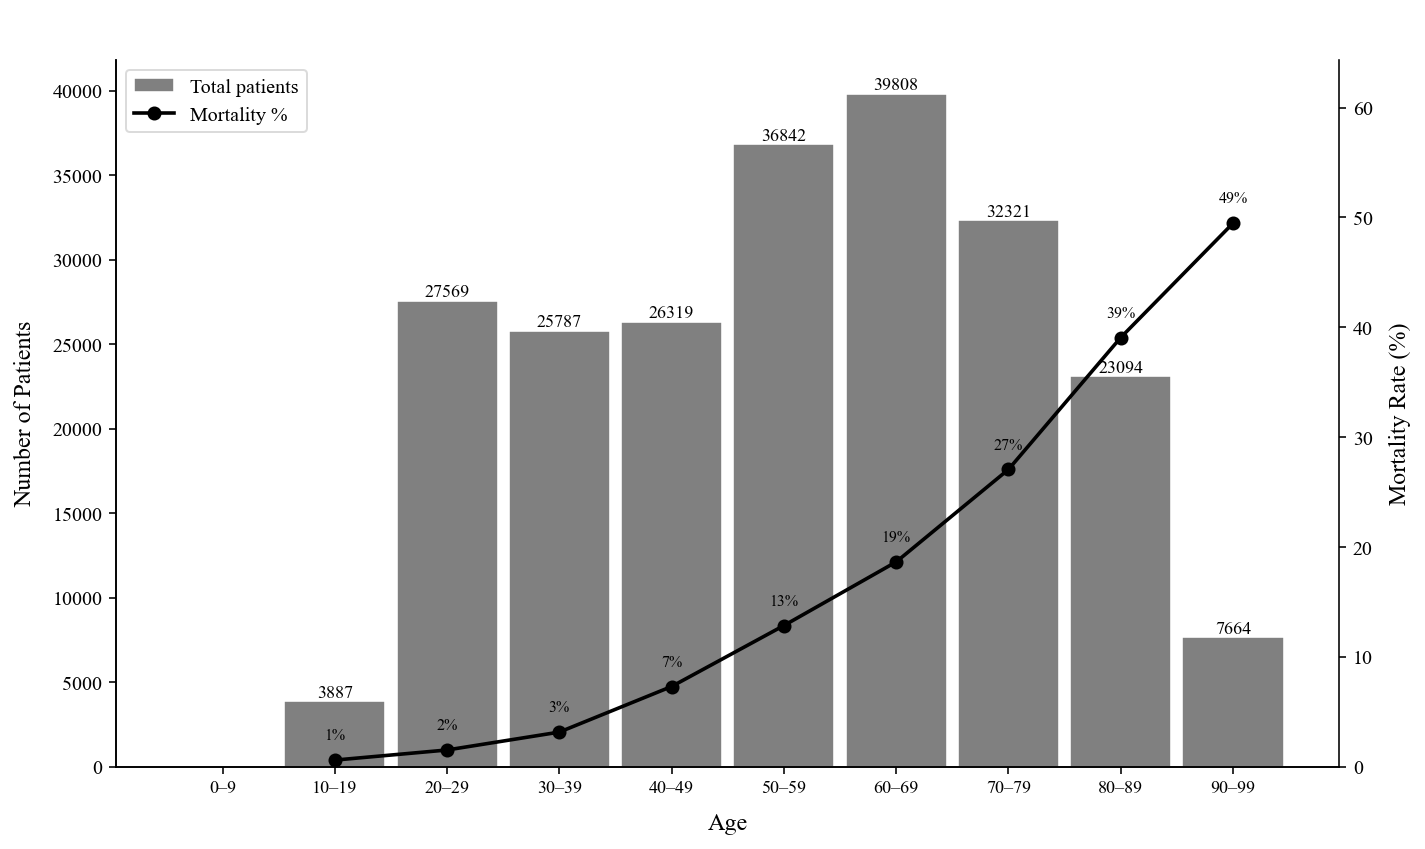
\includegraphics[width=1\textwidth]{hist2.png}
    \caption{Age Distribution and Mortality Rates among Patients in
    Our Dataset}
    \label{fig.age_hist}
\end{figure}

In the dataset, patient ages range from 18 to 91 with an average of
56, and approximately 54\% of patients are younger than 60. Patient
ages are derived from the \texttt{anchor\_age} column in
\texttt{patients.csv}, which caps all ages above 89 at
91~\citep{mimiciv}. Since our threshold of 60 falls below this
ceiling, the cap does not affect the analysis. The age distribution
and mortality rates by age group are shown in
Figure~\ref{fig.age_hist}, using bins
$[0,9],[10,19],\ldots,[80,89],$ $[90,99]$.

We solve problem~\eqref{form.LBBF} with
constraint~\eqref{eq.oldagecon} included in $\calX$ using the hybrid
LBBD algorithm. Constraint~\eqref{eq.zmuLB} is excluded rather than
adjusted, in keeping with our intent to minimize tailoring of the
methodology in the presence of the new constraint.
Table~\ref{tab.Extension} in Appendix~\ref{App.tableDeets} reports
detailed results, summarized in Table~\ref{tab.ExtensionSum}. All
instances across all cohort sizes are solved to optimality.
The addition of this constraint appears to make instances more
tractable compared to the unconstrained results in
Table~\ref{tab.SumH}.

\begin{table}[htbp]
\centering
\resizebox{\textwidth}{!}{\begin{tabular}{rrrrrrrrr}
 \toprule
Size & \multicolumn{2}{c}{Time} & \multicolumn{2}{c}{\#Opt Cuts} &
\multicolumn{2}{c}{\#Feas Cuts} & \multicolumn{2}{c}{\#CBB Cuts}\\
 & Avg & Range & Avg & Range & Avg & Range & Avg & Range\\
\midrule
\numprint{1000} & $<1$ & [$<1$, $<1$] & 5 & [3, 7] & 0 & [0, 0] & 0
& [0, 0]\\
\numprint{5000} & 0 & [0, 1] & 55 & [35, 78] & 34 & [14, 56] & 0 &
[0, 0]\\
\numprint{10000} & 5 & [3, 9] & \numprint{228} & [\numprint{152},
\numprint{273}] & \numprint{189} & [94, \numprint{277}] & 7 & [3,
13]\\
\numprint{15000} & 36 & [12, 45] & \numprint{628} & [\numprint{359},
\numprint{742}] & \numprint{595} & [\numprint{320}, \numprint{769}] &
81 & [27, \numprint{114}]\\
\numprint{20000} & 113 & [89, \numprint{131}] & \numprint{1466} &
[\numprint{1106}, \numprint{1788}] & \numprint{1472} &
[\numprint{948}, \numprint{1921}] & \numprint{290} &
[\numprint{224}, \numprint{350}]\\
\numprint{25000} & \numprint{290} & [\numprint{226}, \numprint{397}] &
\numprint{2724} & [\numprint{2252}, \numprint{3537}] & \numprint{2836}
& [\numprint{2101}, \numprint{3848}] & \numprint{706} &
[\numprint{511}, \numprint{992}]\\
\numprint{30000} & 23 & [18, 29] & \numprint{584} & [\numprint{505},
\numprint{766}] & \numprint{1015} & [\numprint{889},
\numprint{1322}] & 20 & [10, 31]\\
 \bottomrule
\end{tabular}}
  \caption{Summary of Results from the Hybrid LBBD Algorithm with
  Age-Based Side-Constraint}
 \label{tab.ExtensionSum}
\end{table}

Instances with \numprint{15000} patients or fewer are solved in under
one minute. The \numprint{1000}-patient instances are solved in under
1 second using only optimality and feasibility cuts with zero CBB cuts,
and the \numprint{5000}-patient instances in under 1 second on
average. For larger instances, CBB cuts are used more frequently and
running times remain within the time limit, reaching an average of
\numprint{290} seconds at \numprint{25000} patients. For
\numprint{30000}-patient instances, solution times range from 18 to 29
seconds, with an average of 23 seconds.

To examine the effect of the side constraint on the diseases
identified, Tables~\ref{tab.compa6025k} and~\ref{tab.compa6030k}
report the cliques obtained with and without
constraint~\eqref{eq.oldagecon} for the \numprint{25000}-patient and
\numprint{30000}-patient samples, respectively. Results are presented
column-wise for each of the five samples, with ``W/O'' and ``W''
denoting solutions obtained without and with the constraint. Each
table reports the diseases in the clique alongside their
$a_{60}(\cdot)$ values, the mortality rate of the clique, and the
average $a_{60}(\cdot)$ across the clique. Tables~\ref{tab.a60_25k}
and~\ref{tab.a60_30k} in Appendix~\ref{App.tableDeets} summarize the
$a_{60}$ values for all diseases appearing in these tables across the
two cohort sizes. Disease names are abbreviated due to space
limitations; full names are provided in Appendix~\ref{App.Abbs}.

\begin{table}[htbp]
\centering
\resizebox{\textwidth}{!}{
\begin{tabular}{lr|lr|lr|lr|lr|lr|lr|lr|lr|lr}
\toprule
\multicolumn{4}{c|}{Sample \#1} & \multicolumn{4}{c|}{Sample \#2} &
\multicolumn{4}{c|}{Sample \#3} & \multicolumn{4}{c|}{Sample \#4} &
\multicolumn{4}{c}{Sample \#5} \\
\midrule
\multicolumn{2}{c|}{W/O} & \multicolumn{2}{c|}{W} &
\multicolumn{2}{c|}{W/O} & \multicolumn{2}{c|}{W} &
\multicolumn{2}{c|}{W/O} & \multicolumn{2}{c|}{W} &
\multicolumn{2}{c|}{W/O} & \multicolumn{2}{c|}{W} &
\multicolumn{2}{c|}{W/O} & \multicolumn{2}{c}{W} \\
\midrule
Clique & $ a_{60} $ & Clique & $ a_{60} $ & Clique & $ a_{60} $ &
Clique & $ a_{60} $ & Clique & $ a_{60} $ & Clique & $ a_{60} $ &
Clique & $ a_{60} $ & Clique & $ a_{60} $ & Clique & $ a_{60} $ &
Clique & $ a_{60} $ \\
\midrule
OACE & 0.72 & RCU & 0.56 & CA & 0.79 & ONSD & 0.56 & NCD & 0.88 &
PIA & 0.48 & OACE & 0.71 & Hepatitis & 0.28 & SEPT & 0.61 & DCP &
0.58 \\
RF & 0.66 & FevUO & 0.44 & OACE & 0.72 & IntI & 0.54 & OACE & 0.72 &
OLD & 0.47 & HF & 0.79 & OLD & 0.47 & OACE & 0.72 & AlcD & 0.22 \\
PNA & 0.63 & OLD & 0.48 & DLM & 0.73 & MD & 0.38 & AURF & 0.68 & & &
PDX-Unacc & 0.50 & ARenF & 0.71 & DLM & 0.73 & OLD & 0.48 \\
OSNSD & 0.68 & & & RF & 0.66 & & & PDX-Unacc & 0.51 & & & SHK & 0.68
& & & PDX-Unacc & 0.50 & ARenF & 0.71 \\
PDX-Unacc & 0.51 & & & HF & 0.79 & & & OSNSD & 0.67 & & & FED & 0.61
& & & CoagHD & 0.60 & & \\
 &  &  &  & PDX-Unacc & 0.51 &  &  &  &  &  &  &  &  &  &  &  &  &
 &  \\
\midrule
$ \mu $ & Avg & $ \mu $ & Avg & $ \mu $ & Avg & $ \mu $ & Avg & $ \mu
$ & Avg & $ \mu $ & Avg & $ \mu $ & Avg & $ \mu $ & Avg & $ \mu $ &
Avg & $ \mu $ & Avg \\
0.97 & 0.64 & 0.68 & 0.49 & 0.97 & 0.70 & 0.67 & 0.49 & 0.98 & 0.69
& 0.69 & 0.48 & 0.97 & 0.66 & 0.68 & 0.49 & 0.98 & 0.63 & 0.70 &
0.50 \\
\bottomrule
\end{tabular}
}
\caption{Optimal Solutions Found With and Without the Age-Based
Side-Constraint on \numprint{25000}-Patient Samples}
\label{tab.compa6025k}
\end{table}


\begin{table}[htbp]
\centering
\resizebox{\textwidth}{!}{
\begin{tabular}{lr|lr|lr|lr|lr|lr|lr|lr|lr|lr}
\toprule
\multicolumn{4}{c|}{Sample \#1} & \multicolumn{4}{c|}{Sample \#2} &
\multicolumn{4}{c|}{Sample \#3} & \multicolumn{4}{c|}{Sample \#4} &
\multicolumn{4}{c}{Sample \#5} \\
\midrule
\multicolumn{2}{c|}{W/O} & \multicolumn{2}{c|}{W} &
\multicolumn{2}{c|}{W/O} & \multicolumn{2}{c|}{W} &
\multicolumn{2}{c|}{W/O} & \multicolumn{2}{c|}{W} &
\multicolumn{2}{c|}{W/O} & \multicolumn{2}{c|}{W} &
\multicolumn{2}{c|}{W/O} & \multicolumn{2}{c}{W} \\
\midrule
Clique & $ a_{60} $ & Clique & $ a_{60} $ & Clique & $ a_{60} $ &
Clique & $ a_{60} $ & Clique & $ a_{60} $ & Clique & $ a_{60} $ &
Clique & $ a_{60} $ & Clique & $ a_{60} $ & Clique & $ a_{60} $ &
Clique & $ a_{60} $ \\
\midrule
HCSH & 0.79 & RCU & 0.55 & CHF-NH & 0.82 & AlcD & 0.20 & DOA & 0.59
& PS & 0.49 & CardArr & 0.79 & AlcD & 0.21 & HCSH & 0.80 & AlcD &
0.21 \\
ARF  & 0.62 & DOA & 0.59 & DOA    & 0.57 & OLD  & 0.50 & CardArr &
0.79 &      &      & HCSH    & 0.79 & OLD  & 0.51 & SHK  & 0.68 &
OLD  & 0.50 \\
ONSD & 0.56 & AlcD & 0.22 & CUS    & 0.74 &      &      & GD      &
0.59 &      &      & CHF-NH  & 0.82 &      &      & OA   & 0.62 &
&      \\
RCU  & 0.55 &      &      &        &      &      &      & RCU     &
0.57 &      &      & CUS     & 0.73 &      &      &      &      &
&      \\
     &      &      &      &        &      &      &      & CA      &
0.81 &      &      &  &      &      &      &      &      &      &
\\
\midrule
$ \mu $ & Avg & $ \mu $ & Avg & $ \mu $ & Avg & $ \mu $ & Avg & $ \mu
$ & Avg & $ \mu $ & Avg & $ \mu $ & Avg & $ \mu $ & Avg & $ \mu $ &
Avg & $ \mu $ & Avg \\
0.83 & 0.63 & 0.60 & 0.45 & 0.88 & 0.71 & 0.65 & 0.35 & 0.87 & 0.67
& 0.61 & 0.49 & 0.84 & 0.78 & 0.66 & 0.36 & 0.85 & 0.70 & 0.64 &
0.36 \\
\bottomrule
\end{tabular}
}
\caption{Optimal Solutions Found With and Without the Age-Based
Side-Constraint on \numprint{30000}-Patient Samples}
\label{tab.compa6030k}
\end{table}

The solutions obtained without the side constraint show a consistent
pattern: every disease in these cliques has $a_{60}(v) \ge 0.5$,
meaning the majority of its patients are aged 60 or older. For the
\numprint{25000}-patient instances, diseases appearing in the optimal
cliques include neurocognitive disorders ($a_{60} = 0.88$), congestive
heart failure ($a_{60} = 0.79$), coronary atherosclerosis
($a_{60} = 0.79$), disorders of lipid metabolism ($a_{60} = 0.73$),
and other aftercare encounters ($a_{60} = 0.72$). The
\numprint{30000}-patient instances show a similar pattern, with
congestive heart failure ($a_{60} = 0.82$), coronary atherosclerosis
($a_{60} = 0.81$), hypertension with complications ($a_{60} = 0.80$),
and cardiac arrhythmia ($a_{60} = 0.79$) appearing prominently. The
average $a_{60}(\cdot)$ across clique diseases exceeds 0.6 in all
instances, with mortality rates in the range $[0.97, 0.98]$ for the
\numprint{25000}-patient instances and $[0.83, 0.88]$ for the
\numprint{30000}-patient instances, consistent with the values in
Tables~\ref{tab.compa6025k} and~\ref{tab.compa6030k}. These results
indicate that, without the side constraint, the optimal cliques may
reflect the elevated baseline mortality of older patients as much as
the synergistic lethality of co-occurring diseases.

The solutions obtained with the side constraint incorporate diseases
with lower $a_{60}(\cdot)$ values, including alcohol-related disorders
($a_{60} = 0.22$), hepatitis ($a_{60} = 0.28$), mood disorders
($a_{60} = 0.38$), and fever of unknown origin ($a_{60} = 0.44$, as
in Sample~\#1 of Table~\ref{tab.compa6025k}). Mortality rates remain
relatively high at $[0.67, 0.70]$ for the \numprint{25000}-patient
instances and $[0.60, 0.66]$ for the \numprint{30000}-patient
instances. In the presence of the age-based constraint, the
high-mortality cliques frequently include alcohol-related disorders,
other liver diseases, and acute renal failure, consistent with
clinical observations that alcohol-related liver disease co-occurring
with acute kidney injury is associated with elevated short-term
mortality across adult age ranges~\citep{altamirano2012acute}.

\subsection{Case Study: Finding Cancer-Containing
Cliques}\label{sec.CancerSide}

Cancer is among the leading causes of mortality worldwide and
represents a major driver of inpatient mortality in the United
States~\citep{Xu2016}. Within the MIMIC-IV dataset, approximately
20\% of the full cohort, \numprint{44175} of \numprint{223291}
patients, carry at least one cancerous diagnosis, making cancer a
clinically prominent component of the comorbidity landscape. As
illustrated in Figure~\ref{fig.cancer_bar}, the ten most prevalent
cancer diagnoses in the dataset vary substantially in both frequency
and individual mortality rate, with secondary malignancies (SM) and
conditions due to neoplasm or its treatment (CNTN) among the most
lethal. Understanding which non-cancerous diseases co-occur with
cancer to produce the highest joint mortality rates is therefore of
direct clinical relevance for risk stratification and proactive care
planning~\citep{Earle2008, Numico2015}.

\begin{figure}[htbp]
    \centering
    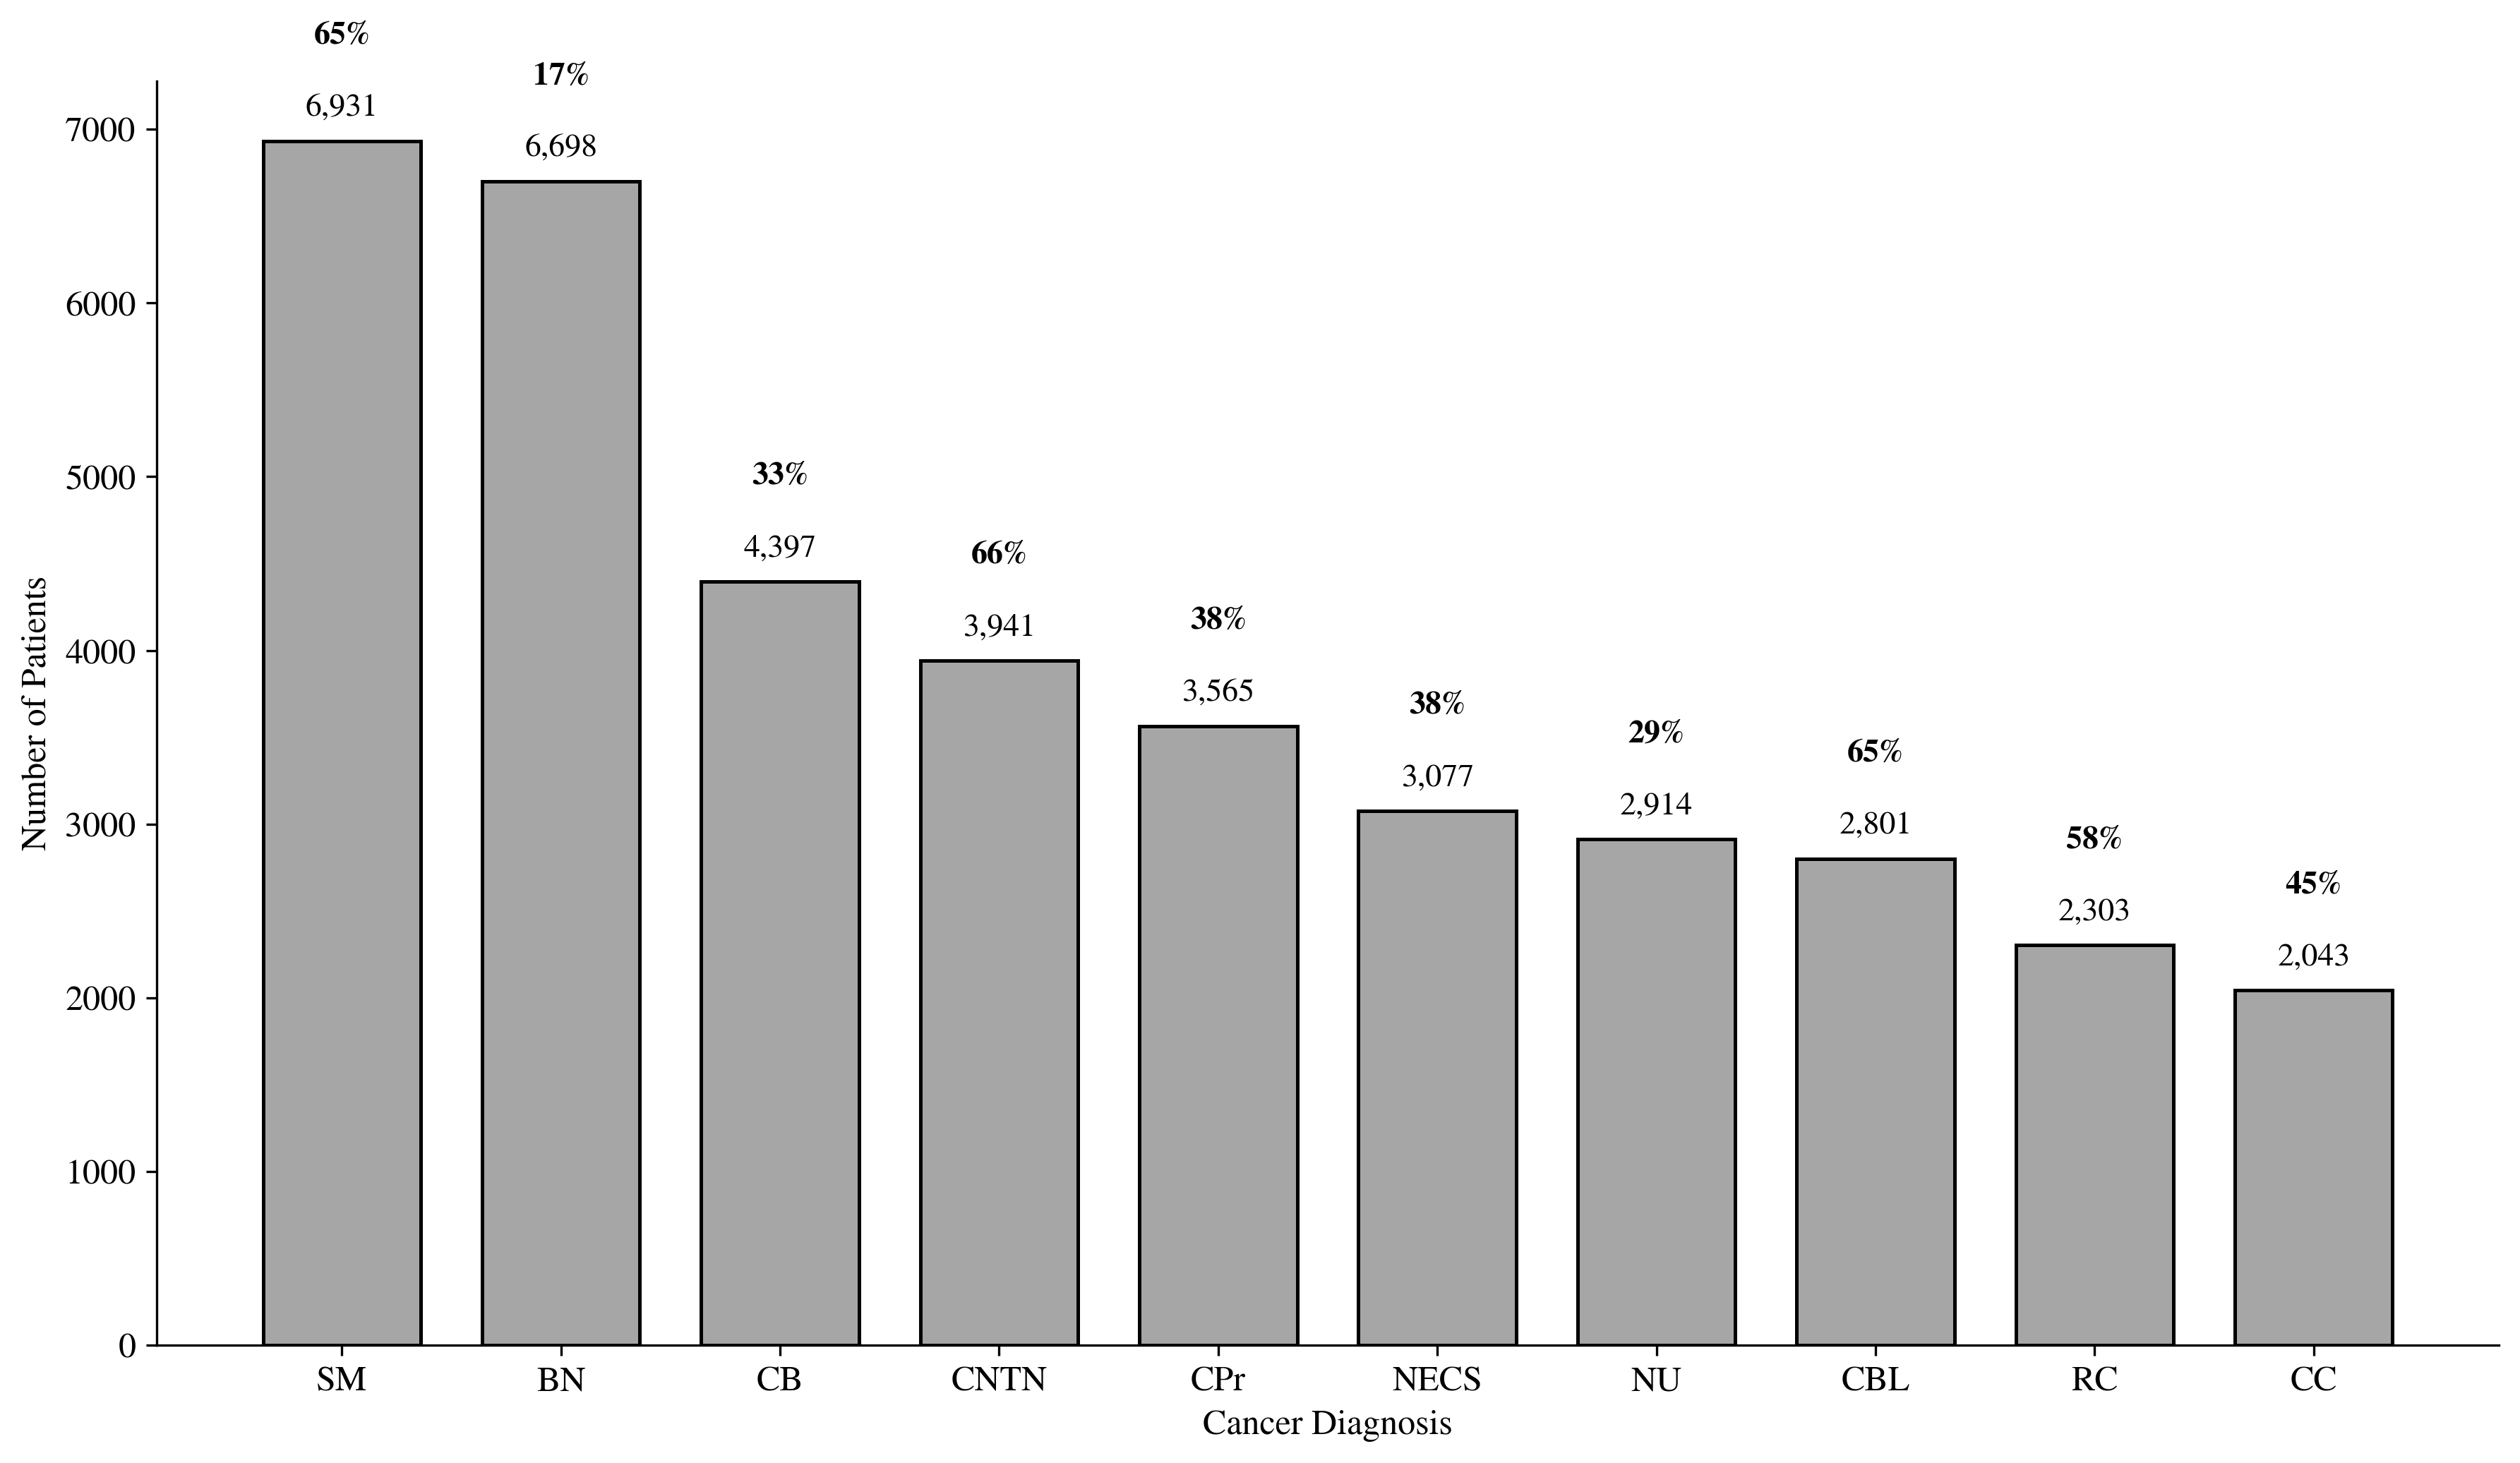
\includegraphics[width=1\textwidth]{top_10_cancers.png}
    \caption{Top-10 Cancer Diagnoses and Their Mortality Rates among
    Patients in Our Dataset}
    \label{fig.cancer_bar}
\end{figure}

We denote by $T$ the set of CCS and CCSR codes corresponding to any
cancerous diagnosis. To identify high-mortality cliques that include
at least one cancer diagnosis, we incorporate the following constraint
into $\calX$:
\begin{equation}\label{eq.Cancon}
    \sum_{v \in T} x_v \;\ge\; 1.
\end{equation}
Constraint~\eqref{eq.zmuLB} is excluded rather than adjusted, in
keeping with our intent to minimize tailoring of the methodology in
the presence of the new constraint. We solve the resulting problem
using the hybrid LBBD algorithm.

Table~\ref{tab.CancerExtension}
summarizes the results across the remaining cohort sizes; detailed
sample-wise results are provided in Table~\ref{tab.cancer_cliques} in
Appendix~\ref{App.tableDeets}. Instances with \numprint{1000} patients are excluded from this case since all five random samples contain no patient carrying a cancerous diagnosis, rendering constraint~\eqref{eq.Cancon} infeasible. 

\begin{table}[htbp]
\centering
\resizebox{\textwidth}{!}{
\begin{tabular}{rrrrrrrrr}
\toprule
Size & \multicolumn{2}{c}{Time} & \multicolumn{2}{c}{\#Opt Cuts} &
\multicolumn{2}{c}{\#Feas Cuts} & \multicolumn{2}{c}{\#CBB Cuts}\\
 & Avg & Range & Avg & Range & Avg & Range & Avg & Range\\
\midrule
\numprint{5000}
& $<1$
& [$<1$, $<1$]
& \numprint{2}
& [\numprint{1}, \numprint{3}]
& \numprint{0}
& [\numprint{0}, \numprint{0}]
& \numprint{0}
& [\numprint{0}, \numprint{0}] \\
\numprint{10000}
& $<1$
& [$<1$, \numprint{1}]
& \numprint{6}
& [\numprint{0}, \numprint{14}]
& \numprint{4}
& [\numprint{0}, \numprint{19}]
& \numprint{0}
& [\numprint{0}, \numprint{0}] \\
\numprint{15000}
& \numprint{2}
& [\numprint{1}, \numprint{2}]
& \numprint{45}
& [\numprint{17}, \numprint{79}]
& \numprint{79}
& [\numprint{4}, \numprint{166}]
& \numprint{0}
& [\numprint{0}, \numprint{0}] \\
\numprint{20000}
& \numprint{29}
& [\numprint{20}, \numprint{42}]
& \numprint{247}
& [\numprint{161}, \numprint{308}]
& \numprint{541}
& [\numprint{360}, \numprint{630}]
& \numprint{13}
& [\numprint{5}, \numprint{26}] \\
\numprint{25000}
& \numprint{61}
& [\numprint{45}, \numprint{78}]
& \numprint{585}
& [\numprint{361}, \numprint{751}]
& \numprint{1087}
& [\numprint{740}, \numprint{1369}]
& \numprint{84}
& [\numprint{40}, \numprint{126}] \\
\numprint{30000}
& \numprint{84}
& [\numprint{65}, \numprint{96}]
& \numprint{1105}
& [\numprint{752}, \numprint{1264}]
& \numprint{1927}
& [\numprint{1420}, \numprint{2199}]
& \numprint{198}
& [\numprint{110}, \numprint{276}] \\
\numprint{223291}
& \numprint{419}
&
& \numprint{1278}
&
& \numprint{41}
&
& \numprint{994}
&  \\
\bottomrule
\end{tabular}}
  \caption{Summary of Results from the Hybrid LBBD Algorithm with
  Cancer-Containing Side-Constraint}
\label{tab.CancerExtensionSum}
\end{table}

In Table~\ref{tab.CancerExtensionSum}, all instances are solved to optimality (0\% gap). The cancer
constraint makes the problem more tractable than the
unconstrained case: the complete dataset that required hundreds of seconds under
the hybrid LBBD without any side constraint (Table~\ref{tab.SumH})
is solved here in a fraction of that time. For cohort sizes up to
\numprint{15000} patients, all instances are solved in under 2
seconds with no CBB cuts required, indicating that the constraint
alone guides the search effectively. CBB cuts begin to contribute at
\numprint{20000} patients (average 13 cuts) and play an increasingly
important role at larger sizes, reaching an average of 198 cuts at
\numprint{30000} patients and 994 cuts on the full
\numprint{223291}-patient instance. The number of optimality and
feasibility cuts grows steadily with cohort size, peaking at averages
of \numprint{1105} and \numprint{1927}, respectively, at
\numprint{30000} patients, before dropping substantially on the full
dataset where the CBB cuts shoulder more of the pruning burden.

To further explore cancer-containing cliques in the complete dataset, we fix exactly one
cancer diagnosis and identify the combination of additional diseases
that maximizes the mortality rate of the resulting clique. We
substitute constraint~\eqref{eq.Cancon} with:
\begin{equation}\label{eq.CanFixcon}
    \sum_{v \in T_{10}} x_v \;=\; 1,
\end{equation}
where $T_{10} = \{\text{SM, BN, CB, CNTN, CPr, NECS, NU, CBL, RC, CC}\}$
denotes the set of the ten most prevalent cancer diagnoses in the
dataset (Figure~\ref{fig.cancer_bar}). For each cancer diagnosis
$C^0 $ from $T_{10}$, we solve problem~\eqref{form.LBBF} with
constraint~\eqref{eq.CanFixcon} and $x_{C^0} = 1$ fixed, effectively
initializing the hybrid LBBD with $C^0$ as the seed clique and
identifying the optimal set of additional diseases $U$ to combine
with it.

\begin{table}[htbp]
\centering
\resizebox{\textwidth}{!}{%
\begin{tabular}{lclcrr}
\toprule
{$C^0$} & \multicolumn{1}{c}{{$\mu(C^0)$}} & {Additional
diseases $U$} & {$\mu(C^0 \cup U)$} & {Increase} & Time\\
\midrule
\multirow{1}{*}{SM} & 0.65 & AURF, CNTN, DLM, OACE, RF, OSS, FED &
1.00 & 54\% & 218 \\
\multirow{1}{*}{BN} & 0.18 & OSNSD, AA, CKD, Hypo, DLM, CoagHD &
0.74 & 331\% & 206 \\
\multirow{1}{*}{CB} & 0.33 & RCU, EsHyp, ONSD, SM, FD & 0.83 &
152\% & 10 \\
\multirow{1}{*}{CNTN} & 0.67 & DLM, SEPT, AURF, AFRD, OACE & 1.00 &
51\% & 135 \\
\multirow{1}{*}{CPr} & 0.38 & CardArr, RCU, GSID, OA, DOA, ARenF &
0.80 & 113\% & 10 \\
\multirow{1}{*}{NECS} & 0.38 & ARenF, CardArr, DOA, FD, RCU, EsHyp,
E-AMD, DLM & 0.86 & 128\% & 27 \\
\multirow{1}{*}{NU} & 0.46 &  & 0.46 & 0\% & 8 \\
\multirow{1}{*}{CBL} & 0.65 & ARF, CardArr, DLM, SM & 0.96 & 48\% &
14 \\
\multirow{1}{*}{RC} & 0.58 & RF, OACE, DLM, PNA & 0.97 & 67\% & 9 \\
\multirow{1}{*}{CC} & 0.45 & GD, SM, RCU & 0.70 & 56\% & 8 \\
\bottomrule
\end{tabular}%
}
\caption{Optimal Cancer-Anchored Cliques Formed by the Addition of
Other Diseases}
\label{tab.cancer_fixed}
\end{table}

Table~\ref{tab.cancer_fixed} reports the results. The individual
mortality rates of the ten cancer diagnoses vary considerably, from
0.18 for benign neoplasms (BN) to 0.67 for conditions due to neoplasm
or its treatment (CNTN), reflecting the well-documented heterogeneity
in prognosis across cancer types~\citep{Earle2008}. The percentage
increase in mortality rate upon adding extra diseases is
inversely related to the baseline cancer mortality: cancers with low
individual mortality (BN at 0.18, CB at 0.33) exhibit the largest
relative gains (331\% and 152\%, respectively), while high-mortality
cancers (CNTN at 0.67, SM at 0.65) show more modest increases (51\%
and 54\%). This pattern suggests that the co-occurring diseases
identified for low-mortality cancers are particularly strong mortality
drivers in combination, rather than independently.

Secondary malignancies (SM) and disorders of lipid metabolism (DLM)
appear as additional diseases across multiple cancer anchors,
suggesting they act as broad comorbidity amplifiers regardless of the
primary cancer type. The co-occurrence of SM with acute and
unspecified renal failure (AURF) and respiratory failure (RF) in the
SM-anchored clique is consistent with the elevated short-term
mortality observed in patients with multi-organ involvement in
advanced malignancy~\citep{Numico2015, Charlson1987}. Similarly, the
combination of CNTN with septicemia (SEPT) and AURF reflects the
well-documented vulnerability of oncology patients to infectious
complications and organ failure during active
treatment~\citep{Kuderer2011}. Respiratory cancers (RC) paired with
respiratory failure (RF), pneumonia (PNA), disorders of lipid
metabolism (DLM), and other aftercare encounters (OACE) reach a
mortality rate of 0.97, consistent with the poor prognosis associated
with advanced lung disease and systemic
compromise~\citep{Niederman2022}.

The SM-anchored and CNTN-anchored cliques both achieve a mortality
rate of 1.00, meaning every patient in the dataset simultaneously
carrying all diseases in these cliques is recorded as expired. While
this reflects the extreme severity of these combinations in the
MIMIC-IV cohort, it should be interpreted cautiously. The
$\ell$-frequency requirement ensures these cliques are supported by
at least $\ell = 100$ patients in the \numprint{223291}-patient
dataset, lending statistical credibility to the finding.

The results of this case study further demonstrate that the hybrid
LBBD framework accommodates cancer-specific constraints without
modification to the core algorithm, and that the resulting
formulation remains tractable across all tested cohort sizes. Full
disease names for all abbreviations used in
Table~\ref{tab.cancer_fixed} are provided in
Appendix~\ref{App.Abbs}.

The results of these two case studies illustrate that the hybrid LBBD framework accommodates side constraints without modification to the core algorithm, and that the resulting formulation remains tractable in practice.

Having established the LBBD framework's flexibility and scalability via decomposition, we now turn to a complementary enumeration-based analysis of small, highly lethal cliques on the full cohort.

\section{Enumeration and Exploring the Comorbidity
Graph}\label{sec.exp2-BKscalability-intro}

The unrestricted MMRCP~\eqref{eq.MMRCP} introduced in Chapter~\ref{sec.probstmnt}
imposes no bound on clique size, reflecting applications in medical
research where restricting attention to small cliques may fail to
capture broader interactions among comorbid diseases that jointly
influence patient outcomes. Alternatively, we can seek an $\ell$-frequent clique of size at most $b$ in the comorbidity
graph $G$ that maximizes the mortality rate. This version focuses
on small but highly lethal disease clusters, which are of particular
value to clinicians assessing future mortality risk in patients with
multiple comorbidities. 

Given a positive integer $b$, the size-restricted problem seeks an
$\ell$-frequent clique $C$ in $G$ with at most $b$ diseases maximizing
$\mu(C)$:
\begin{equation}
    \label{eq.MRP}
    \max\left\{\mu(C) : C \text{ is a nonempty $\ell$-frequent
    clique in } G,\ |C| \le b\right\}.
\end{equation}
The upper bound $b$ ensures that identified clusters are small, as
smaller clusters tend to carry greater diagnostic significance. It is
generally the case that patients with a large number of comorbidities
have higher mortality rates, so restricting $b$ guards against
trivially large cliques driven by that effect. The lower bound $\ell$
ensures that the mortality rate $\mu(C)$ is a statistically reliable
estimate.

A natural variant of problem~\eqref{eq.MRP} is the \textit{maximum
marginal mortality rate clique problem}. Given a pre-established clique
$C^0$ of strictly fewer than $b$ diseases, we seek at most $b -
|C^0|$ additional diseases that maintain the clique property when
added to $C^0$ and maximize the mortality rate of the resulting clique:
\begin{equation}
    \label{eq.margMRP}
    \max\left\{\mu(C) : C \text{ is a nonempty $\ell$-frequent
    clique in } G,\ C \supseteq C^0,\ |C| \le b \right\}.
\end{equation}
This formulation enhances the prognostic potential of the methodology
for patient populations already carrying known diagnoses.
Problem~\eqref{eq.MRP} is a special case of~\eqref{eq.margMRP}
obtained by setting $C^0 = \emptyset$, and both are special cases of
MMRCP~\eqref{eq.MMRCP}.

Algorithm~\ref{alg.MargBKMMRC} in Appendix~\ref{App.Pseudos} solves
both problems~\eqref{eq.MRP} and~\eqref{eq.margMRP} by adapting
the modified BK algorithm (Algorithm~\ref{alg.BKMMRC}) of Section~\ref{sec.MBK} with two changes.
First, the recursion also terminates when $|C| = b$, enforcing the
size bound. Second, rather than tracking a single incumbent, the
algorithm maintains a global max-heap $Q$ prioritized by mortality
rate, into which every $\ell$-frequent clique encountered is inserted.
This allows the top-$K$ highest-mortality cliques to be retrieved for
any positive integer $K$. If $C^0$ is nonempty, it is inserted into
$Q$ initially and the candidate set $L$ is initialized to the common
neighbors of all vertices in $C^0$; otherwise $L = V$. The set
$\texttt{Den}$, representing $\bigcap_{u \in C} A_u$, is tracked
incrementally as in Section~\ref{sec.MBK} to avoid redundant
recomputation.

\subsection{Size-Restricted Most Lethal Cliques}\label{sec.exp2-BKscalability}

The goal of this section is to address problem~\eqref{eq.MRP} and evaluate the performance of the
modified BK algorithm on the complete MIMIC-IV dataset of
\numprint{223291} patient records, which represents the scale at which
the problem is most relevant in practice. Table~\ref{tab.mimicXBK}
presents results for this full dataset. Column ``\#Dec'' records the
number of deceased patients (the numerator of the mortality rate) for
reference, and column ``\#RC'' records the number of recursive calls.
For each value of $b$, we report the top-5 most lethal cliques.

\begin{table}[htbp]
    \small \centering
    {\begin{tabular}{clrrrr}
     \toprule
          $b$ & Clique & \#Dec & $\mu$ & Time & \#RC\\
          \midrule
         \multirow{5}{*}{1} & OACE & \numprint{184636} & 0.83 &
         \multirow{5}{*}{\numprint{1}} &
         \multirow{5}{*}{\numprint{623}} \\
          & CP & \numprint{172829} & 0.77 & & \\
          & GCb & \numprint{165264} & 0.74 & & \\
          & MNWo & \numprint{161972} & 0.73 & & \\
          & ECP & \numprint{156766} & 0.70 & & \\
\midrule
     \multirow{5}{*}{2} & ECP, OACE & \numprint{211396} & 0.95 &
     \multirow{5}{*}{\numprint{4}} &
     \multirow{5}{*}{\numprint{9148}} \\
          & HepF, OACE & \numprint{210706} & 0.94 & & \\
          & AHCD, OACE & \numprint{207341} & 0.93 & & \\
          & SHK, OACE & \numprint{206481} & 0.92 & & \\
          & Coma, OACE & \numprint{206079} & 0.92 & & \\
\midrule
     \multirow{5}{*}{3} & ECP, CNTN, OACE & \numprint{214515} & 0.96 &
     \multirow{5}{*}{\numprint{24}} &
     \multirow{5}{*}{\numprint{136080}} \\
          & ECP, SM, OACE & \numprint{213829} & 0.96 & & \\
          & SHK, HepF, OACE & \numprint{213511} & 0.96 & & \\
          & CD, HepF, OACE & \numprint{213124} & 0.95 & & \\
          & RF, HepF, OACE & \numprint{213076} & 0.95 & & \\
\midrule
     \multirow{5}{*}{4} & SHK, HepF, UTI, OACE & \numprint{218016} &
     0.98 & \multirow{5}{*}{\numprint{119}} &
     \multirow{5}{*}{\numprint{1570449}} \\
          & CD, HepF, UTI, OACE & \numprint{217156} & 0.97 & & \\
          & HP, AMI, OACE, DMWC & \numprint{216818} & 0.97 & & \\
          & HF, HepF, OACE, PNA & \numprint{216799} & 0.97 & & \\
          & HF, Hypo, HepF, OACE & \numprint{216524} & 0.97 & & \\
         \bottomrule
    \end{tabular}}
        \caption{Top-5 Most Lethal Cliques in the \numprint{223291}-Patient
    Dataset Found by Algorithm~\ref{alg.MargBKMMRC}}
    \label{tab.mimicXBK}
\end{table}

Algorithm~\ref{alg.MargBKMMRC} handles the full dataset efficiently across
all values of $b$. Running time grows from 1 second at $b=1$ to 119
seconds at $b=4$, while the number of recursive calls grows from 623
to over 1.5 million, reflecting the increasing combinatorial
complexity with clique size. Among individual diseases ($b=1$), other
aftercare encounter (OACE) has the highest mortality rate at 0.83,
followed by cancer of pancreas (CP) at 0.77 and gastrointestinal
cancers of the bile duct (GCb) at 0.74. As expected, the maximum
mortality rate increases with $b$. At $b=2$, pairing ECP with OACE
yields a rate of 0.95; at $b=3$, the triple \{ECP, CNTN, OACE\}
reaches 0.96; and at $b=4$, the combination \{SHK, HepF, UTI, OACE\}
attains 0.98. The persistent appearance of OACE across all clique
sizes at $b \ge 2$ reflects its frequent co-occurrence with severe
inpatient conditions in the MIMIC-IV dataset. The high mortality rates
associated with hepatic failure (HepF) in combination with shock (SHK)
or cardiac dysrhythmias (CD) are consistent with clinical observations
of poor prognosis in patients with acute-on-chronic liver failure and
hemodynamic instability~\citep{Hernaez2017,Moreau2013}. The recurrence
of cancer-related groups (ECP, CNTN, SM) is in line with elevated
short-term mortality documented in oncology inpatients with advanced
disease~\citep{Earle2008,Numico2015}.

To explore a broader set of disease interactions, we remove from the
\numprint{223291}-patient dataset every patient diagnosed with hepatic
failure (HepF) or other aftercare encounters (OACE), the two conditions
most dominant in Table~\ref{tab.mimicXBK}. The resulting cohort of
\numprint{211391} patients is analyzed using Algorithm~\ref{alg.MargBKMMRC},
and results are reported in Table~\ref{tab.mimicXBKdeletion}.

\begin{table}[htbp]
    \small \centering
    {\begin{tabular}{clrrrr}
          \toprule
         $b$ & Clique & \#Dec & $\mu$ & Time& \#RC\\[0.5ex]
          \midrule
         \multirow{5}{*}{1} & CP & \numprint{163619} & 0.77 &
         \multirow{5}{*}{\numprint{1}} &
         \multirow{5}{*}{\numprint{621}} \\
          & GCb & \numprint{156457} & 0.74 & & \\
          & MNWo & \numprint{153340} & 0.73 & & \\
          & ECP & \numprint{148411} & 0.70 & & \\
          & SM & \numprint{147450} & 0.70 & & \\
\midrule
     \multirow{5}{*}{2} & CAVF, Coma & \numprint{187321} & 0.89 &
     \multirow{5}{*}{\numprint{4}} &
     \multirow{5}{*}{\numprint{9018}} \\
          & ARF, SM & \numprint{180327} & 0.85 & & \\
          & ECP, CNTN & \numprint{179863} & 0.85 & & \\
          & ECP, SM & \numprint{176676} & 0.84 & & \\
          & RF, SM & \numprint{176562} & 0.84 & & \\
\midrule
     \multirow{5}{*}{3} & SM, ARF, PHD & \numprint{192554} & 0.91 &
     \multirow{5}{*}{\numprint{23}} &
     \multirow{5}{*}{\numprint{132907}} \\
          & RF, CNTN, SM & \numprint{190924} & 0.90 & & \\
          & ARF, SM, Phleb & \numprint{190876} & 0.90 & & \\
          & SM, ND, PHD & \numprint{190640} & 0.90 & & \\
          & CAVF, Coma, RF & \numprint{190251} & 0.90 & & \\
\midrule
      \multirow{5}{*}{4} & SHMSA, SM, ARF, PHD & \numprint{199754} &
      0.94 & \multirow{5}{*}{\numprint{118}} &
      \multirow{5}{*}{\numprint{1523191}} \\
          & RC, CNTN, RF, DLM & \numprint{199739} & 0.94 & & \\
          & ARF, SHMSA, SM, Phleb & \numprint{199647} & 0.94 & & \\
          & InjE, SM, DMWC, ARF & \numprint{199647} & 0.94 & & \\
          & CoagHD, NV, PNA, SM & \numprint{198850} & 0.94 & & \\
         \bottomrule
    \end{tabular}}
        \caption{Top-5 Most Lethal Cliques in the \numprint{211391}-Patient
    Dataset Found by Algorithm~\ref{alg.MargBKMMRC}}
    \label{tab.mimicXBKdeletion}
\end{table}

After the exclusion, cancer of pancreas (CP) carries the highest
individual mortality rate at 0.77, followed by GCb at 0.74 and MNWo
at 0.73, the same top three as in Table~\ref{tab.mimicXBK} after
removing OACE. At $b=2$, the pair \{CAVF, Coma\} achieves the highest
pairwise rate of 0.89. Secondary malignancies (SM) feature prominently
across $b \in \{2,3,4\}$, appearing in the majority of top cliques at
each level. At $b=3$, the triple \{SM, ARF, PHD\} reaches 0.91 in 23
seconds with \numprint{132907} recursive calls, and at $b=4$, four of
the five top cliques achieve 0.94 in 118 seconds. Notably, \{SHMSA,
SM, ARF, PHD\} and \{RC, CNTN, RF, DLM\}, the latter involving
respiratory cancers, cancer treatment-related conditions, respiratory
failure, and lipid metabolism disorders, both attain 0.94. The
frequent co-occurrence of SM with pulmonary and hematologic conditions
is consistent with the elevated mortality observed in patients with
multi-organ involvement in advanced
malignancy~\citep{Earle2008,Numico2015,Charlson1987}. The combination
of respiratory cancers with respiratory failure and metabolic
derangement reflects well-documented interactions between advanced
cancer and systemic compromise~\citep{Niederman2022}.

Analyzing the dataset after removing the dominant conditions from
Table~\ref{tab.mimicXBK} reveals a qualitatively different set of
lethal comorbidity patterns, illustrating how the framework can be
used to investigate lesser-known disease combinations. The rapid
escalation of mortality rates with increasing clique size, even among
diseases not individually recognized as acutely lethal, underscores
the value of a systematic comorbidity-aware approach.

\subsection{Marginal Mortality Rate Analysis}\label{sec.exp3-margMR}

The experiments in this section focus on problem~\eqref{eq.margMRP}
with a nonempty $C^0$, using the \numprint{211391}-patient dataset
from Section~\ref{sec.exp2-BKscalability}. For each value of $b$, we
set $C^0$ to be the fifth highest mortality rate clique from
Table~\ref{tab.mimicXBKdeletion}: $C^0 = \{\text{SM}\}$ for $b=1$,
$C^0 = \{\text{RF, SM}\}$ for $b=2$, $C^0 = \{\text{CAVF, Coma,
RF}\}$ for $b=3$, and $C^0 = \{\text{CoagHD, NV, PNA, SM}\}$ for
$b=4$. The results in
Tables~\ref{tab.mimicXBK} and~\ref{tab.mimicXBKdeletion} already
exhibit containment relationships among the top cliques as $b$
increases, so fixing $C^0$ in this way directs the search toward
high marginal mortality cliques not immediately visible from those
tables.

Two experiments are conducted for each $C^0$. In the first,
for each $u \in V \setminus C^0$, we compute $\mu(C^0 \cup
\{u\})$ without requiring $C^0 \cup \{u\}$ to be a clique,
and return the top results by highest marginal mortality rate.
In the second, Algorithm~\ref{alg.MargBKMMRC} is used to find
the highest marginal mortality rate \textit{cliques} containing
$C^0$, allowing the addition of one and then two more diseases.

\begin{table}[htbp]
\centering
\resizebox{\textwidth}{!}{%
\begin{tabular}{lclcrr}
\toprule
{Initial clique $C^0$} & \multicolumn{1}{c}{{$\mu(C^0)$}} & {Additional
disease $u$} & {$\mu(C^0 \cup \{u\})$} & {Increase} & Cluster
type\\
\midrule
\multirow{5}{*}{SM} & 0.70 & Coma & 0.87 & 25\% & 1-defective
clique \\
 & 0.70 & APV & 0.86 & 24\% & 1-defective clique \\
 & 0.70 & CUS & 0.86 & 23\% & 1-defective clique \\
 & 0.70 & ARF & 0.85 & 22\% & clique \\
 & 0.70 & SHK & 0.85 & 21\% & 1-defective clique \\
\midrule
\multirow{5}{*}{RF, SM} & 0.84 & ECP & 0.95 & 13\% & 1-defective
clique\\
 & 0.84 & DOA & 0.92 & 11\% & 2-defective clique \\
 & 0.84 & OLRD & 0.92 & 10\% & 2-defective clique \\
 & 0.84 & DSD & 0.91 & 9\% & 1-defective clique \\
 & 0.84 & PF & 0.91 & 9\% & 1-defective clique \\
\midrule
\multirow{3}{*}{CAVF, Coma, RF} & 0.90 & AURF & 0.91 & 1\% &
1-defective clique\\
 & 0.90 & FED & 0.91 & 1\% & clique \\
 & 0.90 & PDX-Unacc & 0.90 & -1\% & 2-defective clique \\
\midrule
\multirow{2}{*}{CoagHD, NV, PNA, SM} & 0.94 & FED & 0.94 & 1\% &
clique \\
 & 0.94 & PDX-Unacc & 0.94 & 0\% & clique \\[3pt]
\bottomrule
\end{tabular}%
}
\caption{Top-3 Most Lethal Subsets Formed by the Addition of a Single
Disease}
\label{tab.margMRplus1SA}
\end{table}

Table~\ref{tab.margMRplus1SA} reports the results of the first experiment. For each $C^0$, the table lists the additional disease
$u$ yielding the highest, second highest, and third highest increase
in mortality rate, along with the percentage by which
$\mu(C^0 \cup \{u\})$ exceeds $\mu(C^0)$.

When $C^0$ is small, the addition of a single disease can produce
substantial gains. Adding coma to \{SM\} raises the mortality rate
from 0.70 to 0.87 (a 25\% increase), while adding aspiration
pneumonitis (APV) yields 24\%. By contrast, when $|C^0|$ is larger
and $\mu(C^0)$ is already high, marginal gains diminish. For
$C^0 = \{\text{CoagHD, NV, PNA, SM}\}$ with $\mu(C^0) = 0.94$,
addition of FED increases the mortality rate by 1\%.

The column ``Cluster type'' characterizes each subset using the notion
of a \textit{$k$-defective clique}: a vertex set $S \subset V$ is $k$-defective
if the induced subgraph $G[S]$ contains at least $\binom{|S|}{2} - k$
edges, i.e., it falls short of a complete graph by at most $k$ edges.
A standard clique is 0-defective. This characterization is used here
as a natural way to describe near-clique structure; alternative
relaxations such as $k$-plexes~\citep{BBSBIVH11kplex} or
$\gamma$-quasi-cliques~\citep{Pattillo2013qclique} could also be
applied with suitable parameter choices. Three representative examples from
Table~\ref{tab.margMRplus1SA} are visualized in Figure~\ref{fig.defclq123}.

% It is worth noting that an edge in the comorbidity graph reflects
% co-occurrence above threshold $\Delta$ in the EHR dataset.
% Accordingly, for two diseases $u, v \in V$, it is possible that
% $\sigma(u,v) < \Delta$ while $|A_u \cap A_v| \ge \ell$, so a subset
% may contain non-adjacent disease pairs and still correspond to a
% strictly positive mortality rate. The choice of $\ell = 100$ used
% throughout is illustrative; larger values may yield different clusters.

\begin{figure}[htbp]
    \centering
    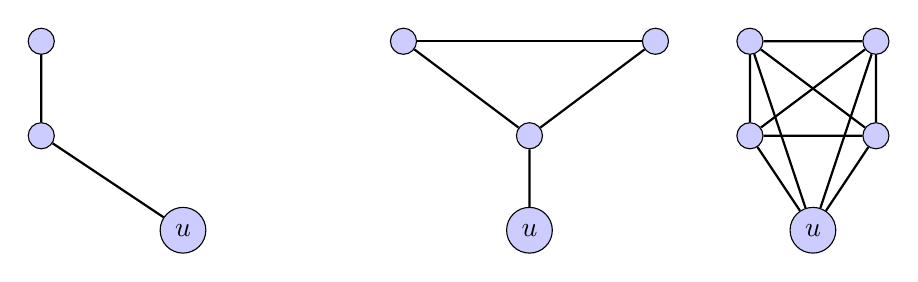
\begin{tikzpicture}
    [scale=.8,auto=left,every node/.style={circle, draw, black,
    fill=blue!20, minimum size = 2pt}]
    \node (n1) at (-1,1){$u$};
    \node (n2) at (-3.25,4)  {};
    \node (n3) at (-3.25,2.5)  {};
    \node (x1) at (4.5,1){$u$};
    \node (x2) at (2.5,4)  {};
    \node (x3) at (4.5,2.5)  {};
    \node (x4) at (6.5,4)  {};
    \node (c1) at (8,2.5){};
    \node (c2) at (8,4)  {};
    \node (c3) at (9,1)  {$u$};
    \node (c4) at (10,2.5) {};
    \node (c5) at (10,4)  {};
    \foreach \from/\to in {n1/n3,n3/n2,
    x1/x3,x2/x3,x2/x4,x3/x4,
    c1/c2,c1/c3,c1/c4,c1/c5,c2/c3,c2/c4,c2/c5,c3/c4,c3/c5,c4/c5}
    \draw[thick] (\from) -- (\to);
    \end{tikzpicture}
    \caption{From left to right, the subgraphs induced by the
    following subsets from Table~\ref{tab.margMRplus1SA}: 1-defective
    clique \{RF, SM, ECP ($u$)\}; 2-defective clique \{CAVF, Coma,
    RF, PDX-Unacc ($u$)\}; clique \{CoagHD, NV, PNA, SM, FED
    ($u$)\}. The added vertex $u$ is labeled in each graph.}
    \label{fig.defclq123}
\end{figure}

Our final experiments assess the performance of
Algorithm~\ref{alg.MargBKMMRC} when initialized with a nonempty $C^0$.
Tables~\ref{tab.margMRplus1t4} and~\ref{tab.margMRplus2t4} report
results complementary to those in Table~\ref{tab.mimicXBKdeletion}
and exhibit trends consistent with Table~\ref{tab.margMRplus1SA}.
These results identify the diseases most consequential to monitor when
a patient already carries a known set of diagnoses, which is the
primary purpose of the marginal mortality rate analysis.

\begin{table}[htbp]
\centering
\resizebox{\textwidth}{!}{%
\begin{tabular}{lclcrrr}
\toprule
{$C^0$} & \multicolumn{1}{c}{{$\mu(C^0)$}} & {Additional disease $u$}
& {$\mu(C^0 \cup \{u\})$} & {Increase} & Time & \#RC \\
\midrule
\multirow{3}{*}{SM} & 0.70 & ARF & 0.85 & 22\% &
\multirow{3}{*}{\numprint{52}} & \multirow{3}{*}{52} \\
 & 0.70 & CP & 0.83 & 20\% & & \\
 & 0.70 & PNAS & 0.83 & 19\% & & \\
\midrule
\multirow{3}{*}{RF, SM} & 0.84 & CNTN & 0.90 & 8\% &
\multirow{3}{*}{\numprint{44}} & \multirow{3}{*}{44} \\
 & 0.84 & Aphleb & 0.89 & 7\% & & \\
 & 0.84 & DKU & 0.89 & 6\% & & \\
\midrule
\multirow{1}{*}{CAVF, Coma, RF} & 0.90 & FED & 0.91 & 1\% &
\multirow{1}{*}{\numprint{2}} & \multirow{1}{*}{2} \\
\midrule
\multirow{2}{*}{CoagHD, NV, PNA, SM} & 0.94 & FED & 0.94 & 0\% &
\multirow{2}{*}{\numprint{3}} & \multirow{2}{*}{3} \\
 & 0.94 & PDX-Unacc & 0.94 & 0\% & & \\[3pt]
\bottomrule
\end{tabular}%
}
\caption{Top-3 Most Lethal Cliques Formed by the Addition of a Single
Disease}
\label{tab.margMRplus1t4}
\end{table}

\begin{table}[htbp]
\centering
\resizebox{\textwidth}{!}{%
\begin{tabular}{lclcrrr}
\toprule
{$C^0$} & \multicolumn{1}{c}{{$\mu(C^0)$}} & {Additional diseases
$u,v$} & {$\mu(C^0 \cup \{u,v\})$} & {Increase} & {Time} &
{\#RC} \\
\midrule
\multirow{3}{*}{SM} & 0.70 & SEPTL, PHD & 0.91 & 31\% &
\multirow{3}{*}{\numprint{787}} & \multirow{3}{*}{\numprint{787}} \\
 & 0.70 & ARF, Phleb & 0.90 & 29\% & & \\
 & 0.70 & ND, PHD & 0.90 & 29\% & & \\
\midrule
\multirow{3}{*}{RF, SM} & 0.84 & DKU, CNTN & 0.94 & 12\% &
\multirow{3}{*}{\numprint{748}} & \multirow{3}{*}{\numprint{748}} \\
 & 0.84 & CNTN, GSS & 0.94 & 12\% & & \\
 & 0.84 & CNTN, SEPT & 0.94 & 12\% & & \\
\midrule
\multirow{1}{*}{CAVF, Coma, RF} & 0.90 & FED & 0.91 & 1\% &
\multirow{1}{*}{\numprint{2}} & \multirow{1}{*}{2} \\
\midrule
\multirow{2}{*}{CoagHD, NV, PNA, SM} & 0.94 & FED, PDX-Unacc & 0.94
& 0\% & \multirow{2}{*}{\numprint{4}} & \multirow{2}{*}{4} \\
 & 0.94 & PDX-Unacc & 0.94 & 0\% & & \\[3pt]
\bottomrule
\end{tabular}%
}
\caption{Top-3 Most Lethal Cliques Formed by the Addition of Two
Diseases}
\label{tab.margMRplus2t4}
\end{table}

Table~\ref{tab.margMRplus1t4} shows that when $C^0 = \{\text{SM}\}$,
adding adult respiratory failure (ARF) yields the largest improvement,
raising its mortality rate from 0.70 to 0.85 (22\%), followed by cancer of
pancreas (CP) and pneumonia (PNAS) at 20\% and 19\%, respectively.
For $C^0 = \{\text{RF, SM}\}$, adding conditions due to neoplasm or
its treatment (CNTN) raises the rate from 0.84 to 0.90 (8\%), with
acute phlebitis (Aphleb) and diseases of kidney and ureters (DKU)
close behind at 7\% and 6\%, respectively. For larger cliques, gains
are marginal: both \{CAVF, Coma, RF\} and \{CoagHD, NV, PNA, SM\}
admit improvements of at most 1\% from any single addition.
Algorithm~\ref{alg.MargBKMMRC} completes all single-addition runs in at
most 52 seconds, confirming its
efficiency when initialized with a nonempty $C^0$.

Table~\ref{tab.margMRplus2t4} reports the results when two diseases
are added simultaneously. Larger gains are possible for smaller
initial cliques: adding SEPTL and PHD to \{SM\} raises the mortality
rate to 0.91 (31\%), and adding DKU and CNTN to \{RF, SM\} raises it
to 0.94 (12\%), each completing in under 790 seconds. For the larger cliques, the maximum gain from any two-disease
addition remains at or below 1\%, consistent with the pattern
observed in Table~\ref{tab.margMRplus1t4}. Together,
Tables~\ref{tab.margMRplus1t4} and~\ref{tab.margMRplus2t4}
demonstrate the utility of the framework for identifying which
additional diseases pose the greatest incremental mortality risk for
a patient already carrying a known set of diagnoses.

Chapter~\ref{sec.conclusion} concludes the dissertation by summarizing contributions, discussing limitations, and outlining directions for future research.